\chapter{METODOLOGIA PROPOSTA}\label{cap:cap3}
O Fluxo de Potência de Segunda Ordem, ou também conhecido na literatura por Fluxo de Potência com Multiplicador Ótimo (\ac{FPMO}), foi originalmente apresentado por Iwamoto e Tamura (\citeyear{iwamoto1981load}) e consiste em uma modificação do método de \acs{NR}.

A principal ideia por trás da modificação é utlizar a expansão de Taylor de segunda ordem para o sistema $F(X)$.
Porém, em sistemas de grande porte como o \acs{SEP}, isso se torna computacionalmente proibitivo dado o custo de armazenar e manipular o tensor Hessiano completo. 

Nesse contexto, é relevante destacar que o método do Multiplicador Ótimo do Fluxo de Potência é uma técnica projetada para contornar a necessidade de calcular e manipular diretamente o tensor Hessiano completo, proporcionando uma abordagem mais eficiente para resolver problemas de otimização em larga escala.

Nesse capítulo, será visto como o método aproxima o tensor Hessiano, permitindo obter a solução para o sistema de equações do \acs{FP}.

\section{FORMULAÇÃO GERAL}

Como dito anteriormente, uma aproximação da expansão de segunda ordem para a função objetivo \ac{FOB} $\Delta F$ é utilizada em \eqref{eq:FX_OM}:
\begin{equation}\label{eq:FX_OM}
    \Delta F \approx \mu J (\Delta X) + \mu^2F(\Delta X)
\end{equation}


A ideia é minimizar a \ac{FOB} com relação a $\mu$, obtendo um valor ótimo de correção do vetor incremento das variáveis de estado, como em \eqref{eq:X_n_OM},  dada uma iteração $n$:
\begin{equation}\label{eq:X_n_OM}
    X_0^{(n+1)} = X_0^{(n)} + \mu \Delta X^{(n)}
\end{equation}

Um detalhe é que $\Delta X^{(n)}$ deve ser obtido da forma tradicional, com a inversa da Jacobiana apenas.
A função objetivo pode ser reescrita de forma simplificada em \eqref{eq:OM_simples}:
\begin{equation}\label{eq:OM_simples}
    a + \mu b + \mu^2c = 0
\end{equation}

Em que, $a$, $b$ e $c$ são obtidos através do conjunto de equações \eqref{eq:a,b,c}:
\begin{equation}\label{eq:a,b,c}
    \begin{split}
        a &= \Delta F \\
        b &= -J \, \Delta X  = -a\\
        c &= -F \, \Delta X
    \end{split}
\end{equation}

Ou seja, o tensor Hessiano é aproximado pelo valor da função avaliado no incremento $\Delta X$, o que facilita sua implementação computacional pelos cálculos já estarem na rotina tradicional do \ac{NR}. A função objetivo que deve ser minimizada é \eqref{eq:FOB_min}, sendo $N$ o número de barras do sistema.
\begin{equation}\label{eq:FOB_min}
    F = \frac{1}{2} \sum_{i=1}^{2N}(a_i +\mu b_i + \mu^2 c_i)^2
\end{equation}

A solução do problema pode ser obtida analiticamente, encontrando as raízes da equação de terceiro grau descrita em \eqref{eq:OM_terceirograu}:
\begin{equation}\label{eq:OM_terceirograu}
    g_0 + g_1 \mu +g_2 \mu^2 + g_3 \mu^3 = 0
\end{equation}

Onde $g_0$, $g_1$, $g_2$ e $g_3$ são dados pelo conjunto de equações \eqref{eq:g0,g1,g2,g3}:
\begin{equation}\label{eq:g0,g1,g2,g3}
    \begin{split}
        g_0 &= \sum_{i=1}^{2N}a_ib_i \\
        g_1 &= \sum_{i=1}^{2N}b_i^2+2a_ic_i \\
        g_2 &= 3\sum_{i=1}^{2N}b_ic_i \\
        g_3 &= 2\sum_{i=1}^{2N}c_i^2
    \end{split}
\end{equation}

Caso o sistema de equações resulte em duas soluções complexas e uma real, escolhe-se sempre a solução real. E caso a solução seja três números reais, escolhe-se a maior solução. A figura \ref{fig:diagrama_FPOM} demonstra em forma de fluxograma como o algoritmo é executado.
\begin{itemize}
    \item Bloco 1: Início do processo;
    \item Bloco 2: Inicializa as variáveis de iterações $n$, o incremento $\Delta X$ e a estimativa inicial para as variáveis de estado $X_0$;
    \item Bloco 3: Calcula o valor da função no ponto de expansão $X_0$;
    \item Bloco 4: Avalia se o valor da função com a estimativa atual é menor ou maior ou igual que o erro máximo aceitável $\epsilon$;
    \item Bloco 5: Caso o valor da função não respeite $\epsilon$, atualiza-se o contador de iterações $n$;
    \item Bloco 6: Avalia se o contador de iterações extrapolou o número máximo de iterações $n_{max}$;
    \item Bloco 7: Calcula a Jacobiana avaliada em $X_0^{n-1}$;
    \item Bloco 8: Com a Jacobiana, calcula o incremento $\Delta X^{n-1}$;
    \item Bloco 9: Calcula os parâmetros $a$, $b$ e $c$ com as equações \eqref{eq:a,b,c};
    \item Bloco 10: Calcula os parâmetros $g_0$, $g_1$, $g_2$ e $g_3$ com as equações \eqref{eq:g0,g1,g2,g3};
    \item Bloco 11: Calcula $\mu$ encontrando as raízes da equação \eqref{eq:OM_terceirograu};
    \item Bloco 12: Atualiza $\Delta X$ considerando o fator multiplicativo $\mu$;
    \item Bloco 13: Atualiza $X_0$ na iteração $n$ com o incremento calculado;
    \item Bloco 14: Caso o valor da função respeite $\epsilon$, o processo finaliza com convergência;
    \item Bloco 15: Caso o número de iterações extrapole o $n_{max}$, o processo se encerra sem uma raíz com erro máximo desejado, indicando divergência.
\end{itemize}
\begin{figure}[H]
    \caption{Fluxograma do método do Multiplicador Ótimo}
    \centering
    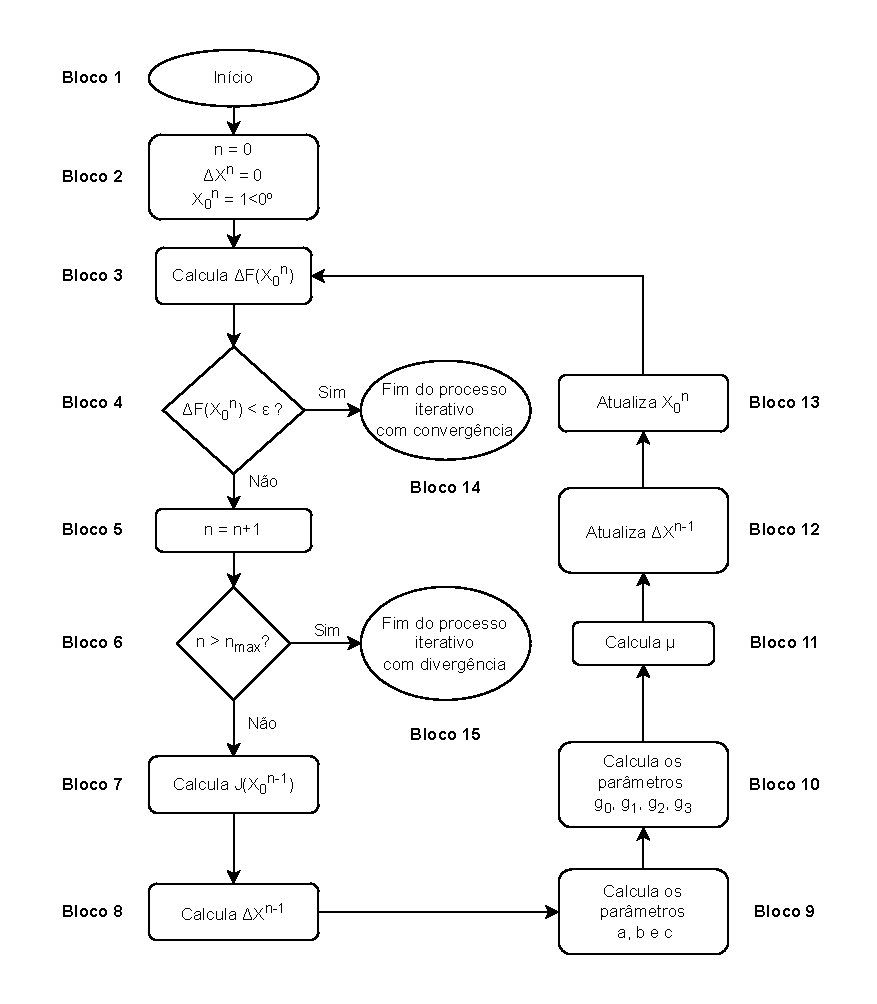
\includegraphics[scale=0.90]{textuais/capitulo3/figuras/Diagrama_NR_OM_5.drawio.pdf}
    \caption*{Fonte: Elaborada pelo autor}
    \label{fig:diagrama_FPOM}
\end{figure}


\section{METODOLOGIA DOS TESTES}
No Capítulo \ref{cap:cap4}, serão apresentados e discutidos os resultados obtidos a partir da aplicação de três variantes apresentadas do método de Newton-Raphson na resolução do problema de \ac{FP}. Os métodos analisados incluem o método em coordenadas retangulares, o método em coordenadas polares e a modificação com Multiplicador Ótimo. O objetivo é comparar a performance e a robustez desses métodos em diferentes cenários, utilizando dois sistemas de teste padrão: o sistema \acs{IEEE} de 14 barras e o sistema \acs{IEEE} de 33 barras. A comparação é realizada com base em 3 testes: carregamento máximo do sistema sem divergência ou soluções espúrias, análise fractal e tempo computacional médio até convergência. 

Todos os experimentos foram realizados em um laptop Acer Nitro 5 com processador Intel Core i5-10300H a 2.50 GHz e 8 GB de RAM, utilizando o sistema operacional Windows 11 Home Single Language, versão 23H2. As simulações foram conduzidas no \textit{software} MATLAB R2021a (9.10.0.1602886). Os testes estão disponíveis no apêndice A.

A metodologia é apresentada a seguir:

\subsection{Carregamento Máximo}
O teste de carregamento máximo visa determinar a fronteira entre a região insolúvel e inviável na situação de aumento sistêmico de carga. O procedimento é detalhado abaixo:
\begin{itemize}
    \item Fator de escala: Definição de um fator de escalonamento $\lambda$ que multiplica as potências ativas e reativas demandadas de todas as barras simultaneamente;
    \item Inicialização: As cargas dos sitemas IEEE 14 e 33 são ajustadas para seus valores base conhecidos, ou $\lambda = 1$, e o erro máximo do \ac{FP} para todas os métodos é definido em  $\epsilon = 10^{-6}$;
    \item Incremento de carga: A carga é aumentada em passos constantes $\Delta \lambda$ até que ocorra a divergência;
    \item Refinamento: Ao detectar divergência, o passo do incremento é reduzido e o fator $\lambda$ é refinado;
    \item Análise: Os fatores de carregamento máximos alcançados por cada método são comparados.
\end{itemize}
\subsection{Análise Fractal}
É conhecido na literatura que as múltiplas soluções do método de \ac{NR} são fractalizadas, isto é, apresentam uma fronteira fractal em sua região de convergência. Isso implica que pequenas variações nas estimativas iniciais próximas à fronteira de convergência podem levar a soluções diferentes do fluxo, como evidenciado por Thorp (\citeyear{thorp}) e Deng et al. (\citeyear{convergence_region}).

Os fractais são construídos plotando-se em um gráfico, onde os eixos representam as variáveis de estado de um problema. Cada par ordenado indica um palpite inicial para o processo e é colorido com base nas diferentes soluções possíveis. Até mesmo pares ordenados que não levam a nenhuma solução podem ser inseridos no mapa em uma determinada cor.

Por isso, plotar os fractais de cada método avaliado pode ser uma ferramenta visual e eficaz capaz de avaliar a robustez do algoritmo considerando sua capacidade de convergência para palpites iniciais diversos. 

Os fractais de Newton para o \ac{FP} teriam uma dimensão igual ao número de variáveis, o que tornaria impossível a representação visual em uma figura \acs{2D}. Uma alternativa é construir um algoritmo que execute diversas combinações de tensão e ângulo como palpites iniciais, mas para todas as barras de forma idêntica. Assim, é possível construir um único fractal \acs{2D} que permitirá a comparação do tamanho da região de convergência dos três métodos.

O teste será conduzido da seguinte forma:
\begin{itemize}
    \item Rodar o \ac{FP} polar, retangular e \ac{FPMO} em carga nominal, média e próxima ao \ac{PMC} com estimativas iniciais de $1\angle 0 ^{\circ}$ e armazenar os valores de tensão e ângulo para cada uma das cargas;
    \item Estabelecer uma faixa de valores que serão iterados os ângulos e fases e rodar o fluxo repetidamente para cada combinação de estimativas iniciais;
    \item Comparar as soluções com a solução previamente calculada;
    \item Se as soluções obedecerem a um erro estabelecido, serão consideradas estáveis; caso contrário, instáveis;
    \item Plotar em um gráfico, utilizando a cor azul para soluções estáveis e vermelho para instáveis;
    \item Analisar as regiões de cada método e compará-las.
\end{itemize}

\subsection{Tempo Computacional e número de iterações}
O teste de tempo computacional visa comparar a eficiência dos métodos em termos de tempo de execução. Medir o tempo necessário para resolver o problema de fluxo de potência é crucial para avaliar o desempenho prático dos algoritmos. Este teste é fundamental para determinar a viabilidade de uma técnica em aplicações de curto prazo, como a operação em tempo real do \ac{SIN}. A descrição da metodologia utilizada está abaixo:

\begin{itemize}
    \item Os algoritmos serão rodados repetidamente nos sistemas teste em carga nominal;
    \item Serão armazenados os tempos e iterações médios do \ac{FP};
    \item Os dados obtidos serão analisados e comparados;
\end{itemize}